\chapter{بازی \lr{Pacman}}
\section{مقدمه}
\par
بازی ها یکی از مهم ترین زمینه هایی هستند که هوش مصنوعی توانسته است با قدرت در آن ها نفوذ نموده و جای یازیکن های انسانی را بگیرد . بازیکن، کنترل پَک-مَن را در یک هزارتو (\footnote{\lr{Maze}}) بر عهده دارد که در این هزارتو باید به خوردن نقطه‌ها بپردازد. دشمنان بازی پَک-مَن با اصطلاح‌های مختلفی مانند «روح‌ها»، «گابلین‌ها»، «اُختاپوس‌ها» و «هیولاها» شناخته می‌شوند.
\begin{figure}[h]
	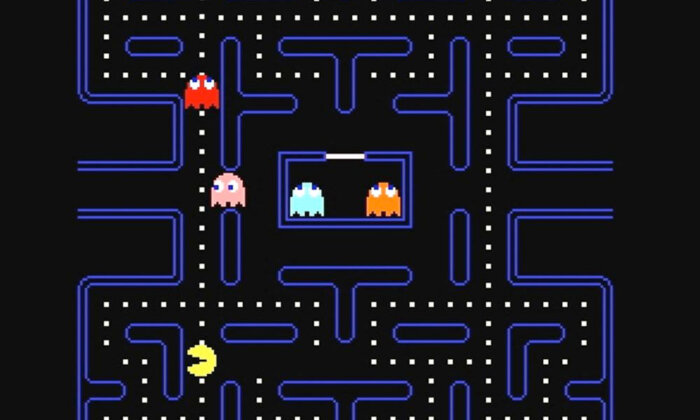
\includegraphics[scale=0.6]{pacman}
	\centering
	\caption{بازی \lr{pacman}}
	\cite{NoahWardrip}
	\label{fig2}
\end{figure} 
\section{طرح مسئله}
زیمن بازی از یک صفحه 9 در 18 درست شده است که موانع جوایزی درزمین بازی قرار گرفته شده اند . در این بازی باید با استفاده از الگوریتم 
\lr{min-max}
باید عامل هوشمند تصمیم بگیرد تا 
\lr{Pacman}
را در کدام جهت هدایت نماید . محیط بازی به صورت پویا ست و همین طور حرکت روح ها به صورت تصادفی می باشد . عامل هوشمند فرض را بر این می گذارد که در هر گام حریف یعنی روح ها بهینه ترین کار برای خودشان را انجام می دهند . در هر گام عامل با توجه به ارزش گذاری فضای حالات تصمیم می گیرد که در کدام جهت حرکت نماید . همین طور به علت این که نمی تون تا هر عمق دلخواهی در درخت حالات جست و جو نمود بایستی تابع ارزیابی طرح نمود تا بتوان با استفاده از آن خوب بودن یک حالت را بررسی نمود .

\section{لینک گیت هاب کد}
با مراجعه به 
\url{https://github.com/mahdialipoo/AI_AUT_Project3}
می توانید کد مربوط به پیاده سازی این بازی را مشاهده نمایید .
